\section{Introduction}
\label{sec:intro}
% 1.Background
%% 1.1 RGB Video Generation
Text-to-Video generative models have quickly advanced, achieving impressive results~\cite{he2022latent, chen2023videocrafter1, guo2023animatediff, wang2023modelscope, wang2024videocomposer, zhang2023show, yang2024cogvideox, opensora, opensoraplan}. This progress has enabled various applications, such as video editing~\cite{geyer2023tokenflow, yang2023rerender, qi2023fatezero, liu2024video, wu2023tune, chen2023control}, image animation~\cite{blattmann2023stable, niu2024mofa, guo2024liveportrait, guo2023i2v}, and motion customization~\cite{he2024cameractrl, wang2024motionctrl, ling2024motionclone, jeong2024dreammotion, ma2023trailblazer, yin2023dragnuwa, wang2024motion}. Diffusion Transformers (DiT) enhance these models by using self-attention to capture long-range dependencies~\cite{sora2024, opensora, opensoraplan, yang2024cogvideox}. These models are now widely used in entertainment, advertising, and education, meeting the demand for customizable, dynamic content. 
Notably, Text-to-RGBA (A denotes Alpha channel) video generation is invaluable for VFX and creative industries. The inclusion of an alpha channel in RGBA formats allows for transparent effects, enabling seamless blending of elements like smoke and reflections (see Fig.~\ref{fig:teaser}). This transparency creates realistic visuals that can integrate smoothly into scenes without modifying the background. Such flexibility is crucial in gaming, virtual reality (VR), and augmented reality (AR), where dynamic and interactive content is in high demand.


% 2. Research Gap
%% 2.1 Limited Data - Text & Motion Diversity, Gap between RGB Data and RGBA Data -> Need for RGB Generation Prior
Currently, no direct solutions exist for RGBA video generation, which remains a challenging task due to the scarcity of RGBA video data, with only around 484 videos available in~\cite{lin2021real}. This scarcity will significantly limit the diversity of generated content, resulting in a constrained set of object types and motion patterns.
One feasible solution is to use video matting~\cite{qin2023bimatting,lin2022robust,lin2023omnimatterf} to obtain alpha channels from generated videos. However, these methods are still limited by the scarcity of RGBA video data and struggle to generalize to a wider range of objects, as shown in Fig.~\ref{fig-intro} (b).
Other video segmentation methods, such as SAM-2~\cite{ravi2024sam2}, may generalize well to different tasks. However, they cannot generate alpha channels and are therefore unsuitable for direct compositing.
There have been attempts to generate RGBA at the image level, such as LayerDiffusion~\cite{zhang2024transparent}. 
However, adapting its concept directly to a temporal VAE used in video generative models remains challenging.

In this paper, we explore how to extend pretrained video models to generate corresponding alpha channels while retaining the original capabilities of pretrained models. Our goal is to generate content beyond the limitations of the current RGBA training set.
Existing works such as Lotus~\cite{he2024lotus} and Marigold~\cite{ke2024repurposing} demonstrate that leveraging pretrained generation model weights significantly enhances out-of-distribution in dense prediction, hinting at the potential for predicting alpha channels.
% However, these approaches leave room for improvement as they keep RGB generation and alpha prediction largely separate, with information flowing only from RGB to alpha. 
However, in the context of RGBA video generation, these approaches typically require generating RGB channels first, followed by separate alpha channel prediction. Consequently, information flows unidirectionally from RGB to alpha, keeping the two processes largely disconnected.
Given the limited availability of RGBA video data, this imbalance results in insufficient alpha prediction when challenging objects are generated, as shown in Fig.~\ref{fig-intro} (c).

\begin{figure}[t]
    \centering
    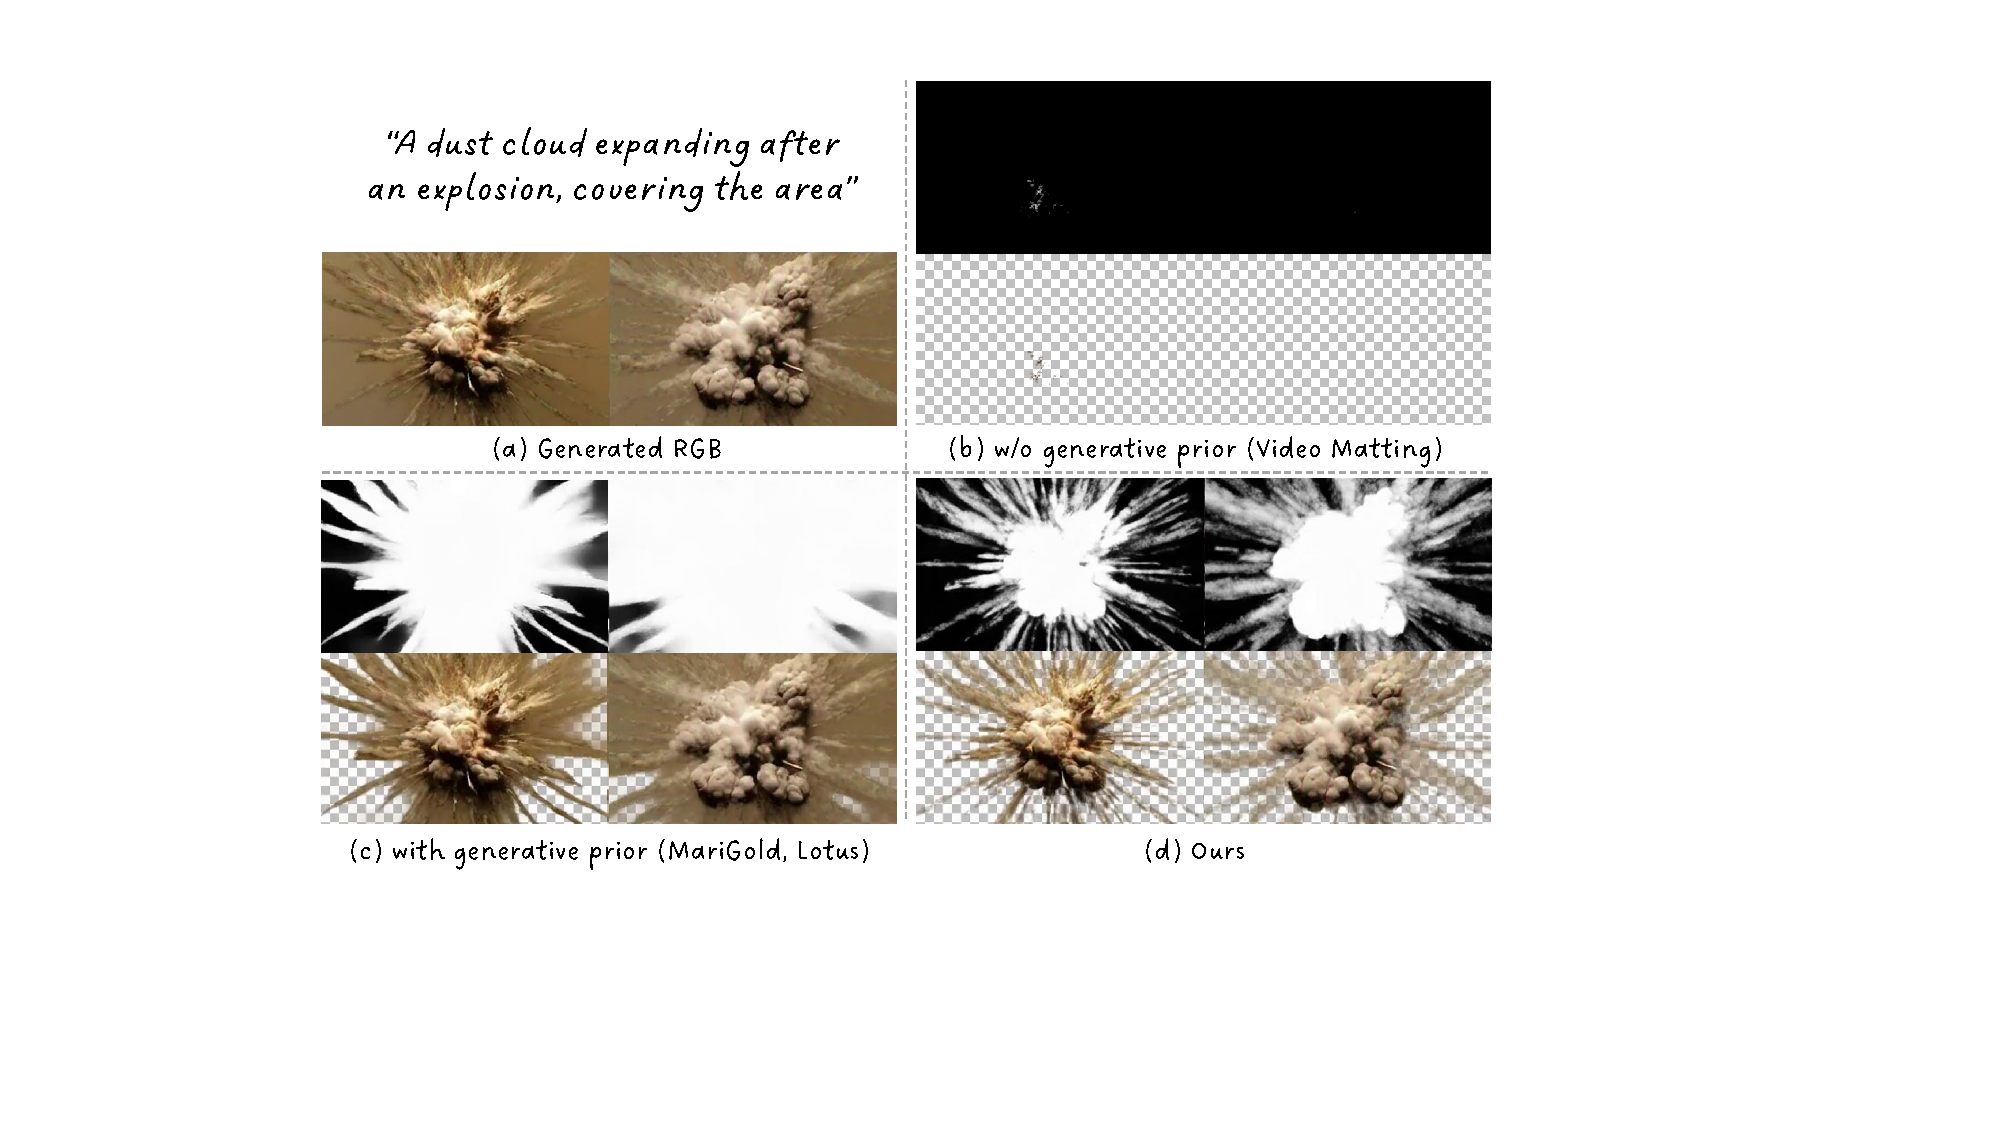
\includegraphics[width=1.0\linewidth]{figs/intro.pdf}
    \vspace{-0.2in}
    \caption{Comparison between \textbf{Generation-Then-Prediction} and our \textbf{Joint Generation} approach. Given the generated RGB in (a), (b) and (c) show the predicted alpha (top) and the composited result (bottom). In (d), the top shows the jointly generated alpha.}
    \label{fig-intro}
    \vspace{-0.2in}
\end{figure}

In this work, we propose \textbf{TransPixar}, which effectively adapts the pretrained RGB video models to generate RGB channels and the alpha channel simultaneously. 
%Since RGB and alpha are jointly generated, this approach maximizes consistency between them.
We leverage state-of-the-art DiT-like video generation models~\cite{yang2024cogvideox, opensoraplan} 
%which combined text and RGB tokens into a long sequence
%and apply self-attention across them. On top of that, 
, and additionally introduce new tokens appended after text and RGB tokens %which matches the length of the RGB tokens and are decoded into 
for generating the alpha channels. 
%
To facilitate convergence, we reinitialize the positional embeddings for the alpha tokens and introduce a zero-initialized, learnable domain embedding to distinguish alpha tokens from RGB tokens. Furthermore, we employ a LoRA-based fine-tuning scheme~\cite{hu2021lora}, applied exclusively to project alpha tokens into the qkv space, thereby maintaining RGB generation quality.
With the proposed approach, we extend the modality while preserving the original input-output structure and relying on the existing attention mechanism through LoRA adaptation. 
%This effectively integrates new functionality without significant changes to the architecture.

The extended sequence contains text, RGB, and alpha tokens, with self-attention divided into a 3x3 grouped attention matrix involving interactions like \textbf{Text-attend-to-RGB} (Text as query, RGB as key) and others. 
We also systematically analyze the attention mechanisms for RGBA generation: 1) \textbf{Text-attend-to-RGB} and \textbf{RGB-attend-to-Text}. The interaction between text and RGB tokens represents original model's generation capabilities. Minimizing the impact on text and RGB tokens during these attention computation processes can better retain the original model's performance;
2) \textbf{RGB-attend-to-Alpha}. We reveals a fundamental limitation in conventional methods is the lack of \textbf{RGB-attend-to-Alpha} attention. This attention is necessary to refine RGB tokens based on alpha information, improving RGB-alpha alignment; 3) \textbf{Text-attend-to-Alpha}. We remove this attention mechanism to reduce the risk caused by limited training data, which could degrade the model's performance. This removal also enhances the retention of the model's original capabilities.

By integrating these techniques, our method achieves diverse RGBA generation with limited training data while maintaining strong RGB-alpha alignment. To summarize, our contributions are as follows:
\begin{itemize}
    \item We propose an RGBA video generation framework using DiT models that requires limited data and training parameters, achieving diverse generation with strong alignment.
    \item We analyze the role of each attention component in the generation process, optimize their interactions, and introduce necessary modifications to improve RGBA generation quality.
    \item Our method is validated through extensive experiments, demonstrating its effectiveness across a variety of challenging scenarios.
\end{itemize} 


% To enable Text-to-RGBA video generation, one of the primary challenges is the scarcity of large-scale, high-quality RGBA video datasets. Compared to the abundance of Text-to-RGB data~\cite{schuhmann2022laion}, available RGBA datasets~\cite{lin2021real, tudosiu2024mulan} are much smaller, and RGBA video data is even rarer, with only around 484 videos in~\cite{lin2021real}. 
% This data shortage limits both motion diversity and the ability to generate RGBA videos from diverse text prompts—factors crucial for high-quality RGBA generation. 
% As illustrated in Fig.~\ref{fig-intro}, with limited data, the straightforward solution—applying video matting~\cite{qin2023bimatting,lin2022robust,lin2023omnimatterf} to obtain alpha channels—often falls short, as these methods struggle to generalize to non-human object categories.
% To overcome this limitation, leveraging existing RGB generation models is an effective approach, as they are trained on large datasets and exhibit strong generalization capabilities. 
% For example, some methods focus on transforming pretrained RGB generation models~\cite{ke2024repurposing, he2024lotus, yang2024depth} into prediction models, such as by predicting the alpha channel, enabling RGBA generation through a generation-then-prediction process. As shown in our work, these methods often outperform traditional video matting techniques~\cite{chen2022pp, li2024matting, yao2024vitmatte, wang2024matting}. However, they still face challenges with out-of-distribution (OOD) samples, as illustrated in Fig.~\ref{fig-intro}. When the generated RGB video falls outside the expected distribution, the model's alpha prediction accuracy significantly declines, making this approach unstable for complex VFX use cases.
% Alternatively, other approaches focus on adapting pretrained RGB generation models directly into RGBX generation models~\cite{long2024wonder3d, zeng2024rgb, zhang2024transparent}. This joint-generation strategy avoids OOD issues and enhances alignment between RGB and alpha channels. 
% However, when applied to video generation with limited training data, these models still struggle to meet the demands of more creative tasks that require fine-grained visual fidelity.

% % 3. Our Solution
% In this work, we present a method to extend an RGB generation model to support RGBA generation while preserving RGB generation potential. 
% Our research leverages the latest DiT-like video generation models~\cite{yang2024cogvideox, opensoraplan}. 
% % RGBA image data
% The core process of these models involves concatenating text and RGB tokens into a long sequence and applying self-attention across them.
% Building upon this foundation, we append a series of new tokens after text and RGB tokens during generation.
% These tokens match the length of RGB tokens and will be decoded into corresponding alpha channels after generation. 
% Specifically, we reinitialize the positional embeddings for alpha tokens to improve training convergence and introduce a zero-initialized, learnable domain embedding to differentiate alpha tokens from RGB tokens.
% We also propose a fine-tuning scheme based on LoRA~\cite{hu2021lora}. To maintain RGB generation potential, we apply LoRA only when projecting alpha tokens into the qkv space, preserving RGB generation quality.

% %% 3.2 Attention Rebias - (Text -> Alpha)
% Since the most critical computation in the DiT model is attention, we analyze the attention mechanisms involved in the RGBA generation process.
% The newly extended sequences include text, RGB, and alpha tokens, with self-attention divided into a 3x3 grouped attention matrix—\textbf{Text-to-RGB}, \textbf{RGB-to-Text}, etc. 
% Our analysis revealed that the prediction methods faces a fundamental limitation due to the lack of crucial \textbf{RGB-to-Alpha} attention.
% This attention is essential for refining RGB tokens based on alpha information, allowing for better RGB-alpha alignment.
% To further streamline the model, we remove unnecessary attention computations, such as \textbf{Text-to-Alpha}, since alpha tokens contain contour information only. They lack the color, texture, and semantics typically described in text tokens, and text-to-alpha attention would degrade the final generation quality.
% By combining these techniques, our method achieves diverse RGBA generation with limited training data while maintaining strong alignment.
%





